% \documentclass{template/openetcs_article}

% \usepackage{graphicx}

% %\usepackage[top=3cm, bottom=2.5cm, left=3cm, right=2.5cm] {geometry}
% \usepackage {bsymb,b2latex}
% \usepackage{b2latex}
% \usepackage{fancyhdr}
% %\usepackge{lastpage}%
% %\usepackge{color}
% \graphicspath{{./template/}{.}{./images/}}
% %\usepackage[utf8]{inputenc}

%---------------------------------------------------------

\documentclass{template/openetcs_article}
% Use the option "nocc" if the document is not licensed under Creative Commons
%\documentclass[nocc]{template/openetcs_article}
\usepackage {bsymb,b2latex}
\usepackage{lipsum,url,color}
\graphicspath{{./template/}{.}{./images/}}
\begin{document}
\frontmatter
\project{openETCS}

%Please do not change anything above this line
%============================
% The document metadata is defined below

%assign a report number here
\reportnum{OETCS}

%define your workpackage here
\wp{Work-Package 7: ``Toolchain''}


\newcommand{\true}{\ensuremath{true}}
\newcommand{\btext}[1]{{\it #1}}
\newcommand{\bvar}[1]{\btext{#1}}
\newcommand{\bevent}[1]{\btext{#1}}
\newcommand{\binv}[1]{\btext{#1}}
\newcommand{\bconst}[1]{\btext{#1}}
\newcommand{\bparam}[1]{\btext{#1}}
\newcommand{\bfunc}[1]{\btext{#1}}
\newcommand{\baxiom}[1]{\btext{#1}}
\newcommand{\btype}[1]{\btext{#1}}
\newcommand{\bguard}[1]{\btext{#1}}
\newcommand{\bmachine}[1]{\btext{#1}}
\newcommand{\bctx}[1]{\btext{#1}}

\author{Matthias Güdemann\\Systerel, France}

\affiliation{Systerel}

\title{Event-B Model of Subset 026, Section 5.9}

% define the coverart
\coverart[width=350pt]{chart}

\reporttype{Model Description}

%\begin{document}

\maketitle
\tableofcontents
\listoffiguresandtables
\newpage

This document describes a formal model of the requirements of section~5.9 of
the subset 026 of the ETCS specification 3.3.0~\cite{SRS-026-330}. This section
describes the on-sight procedure.

The model is expressed in the formal language Event-B~\cite{abrial-eventB-Book}
and developed within the Rodin tool~\cite{rodin-handbook}. This formalism allows
an iterative modeling approach. In general, one starts with a very abstract
description of the basic functionality and step-wise adds additional details
until the desired level of accuracy of the model is reached. Rodin provides the
necessary proof support to ensure the correctness of the refined behavior.

In this document we present an Event-B model of the procedure on-sight. We use
the iUML plugin which allows for modeling in UML state-charts to create a
graphical model of the procedure which is as close as possible as its
description as flowchart in the section 5.9. The state machine is iteratively
developed using the refinement feature of Event-B. At each refinement step, we
present the reasoning for the step, together with newly introduced variables and
events.

\begin{table}[ht]
  \centering
  \begin{tabular}[ht]{|l|l|}
    \hline
    \hline
  \end{tabular}
  \caption{Glossary}
  \label{tab:glossary}
\end{table}

\section{Short Introduction to Event-B}
\label{sec:short-intr-event}

The formal language Event-B is based on a set-theoretic approach. It is a
variant of the B language, with a focus on system level
modeling~\cite{abrial-eventB-Book}. An Event-B model is separated into a static
and a dynamic part.

The dynamic part of an Event-B model describes abstract state machines. The
state is represented by a set of state variables. A transition from one state to
another is represented by parametrized events which assign new values to the
state variables. Event-B allows unbounded state spaces. They are constrained by
invariants expressed in first order logic with equality which must be fulfilled
in any case. The initial state is created by a special initialization event.

The static part of an Event-B model is represented by contexts. These consist of
carrier sets, constants and axioms. The type system of a model is described by
means of carrier sets and constraints expressed by axioms.

Event-B is not only comprised of descriptions of abstract state machines and
contexts, but also includes a development approach. This approach consists of
iterative refinement of the machines until the desired level of detail is
reached. In the Rodin tool, proof obligations are automatically created which
ensure correct refinement.

Together with the machine invariants, the proof obligations for the refinement
are formally proven, creating proof trees. To accomplish this, there are
different options: many proof obligations can be discharged by automated provers
(e.g., AtelierB, NewPP, Rodin's SMT-plugin), but as the underlying logic is in
general undecidable, it is sometimes necessary to use the interactive proof
support of Rodin.

Any external actions, e.g., mode changes by the driver or train level changes
are modeled via parametrized events. Only events can modify the variables of a
machine. An Event-B model is on the system level, events are assumed to be
called from a software system into which the functional model is embedded. The
guards of the events assure that any event can only be called when appropriate.

\section{Modeling Strategy}
\label{sec:modeling-strategy}

The section~5.9 of the SRS describes the procedure on-sight, in particular it
describes the sequence of mode changes, necessary driver acknowledge and train
brake to enter OS mode, dependent on the current train mode.

For better understanding and to automate many tasks for state based modeling, we
use the iUML plugin~\cite{UML-plugin} which automatically generates Event-B code
representing a state machine specification.

\section{Model Overview}
\label{sec:model-overview}

Figure~\ref{fig:model-overview} shows the structure of the Event-B model. The
left column represents the abstract state machines, the right column the
contexts. An arrow from one machine to another machine represents a refinement
relation, an arrow from a machine to a context represents a sees relation and
arrow from one context to another represents an extension relation.

\begin{figure}[ht]
  \centering
  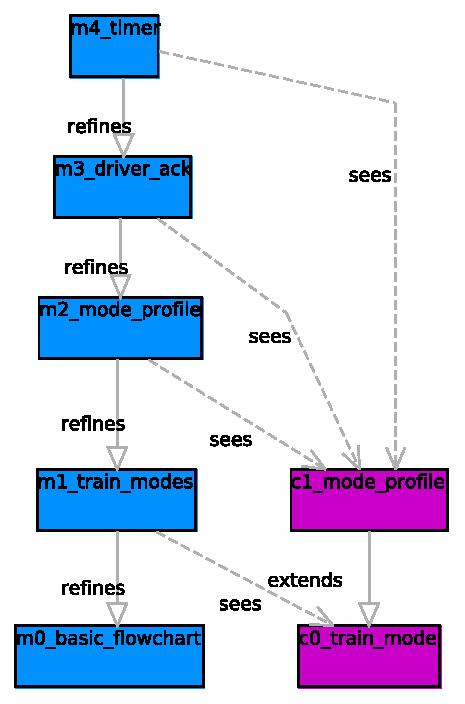
\includegraphics[width=.3\textwidth]{SubSet_026_5_9}
  \caption{Overview on State Machine and Context Hierarchy}
  \label{fig:model-overview}
\end{figure}

The modeling starts with the very abstract possibility to establish and to
terminate a communication session in the machine \bmachine{m0}, the set of
entities is defined in the context \bctx{c0}. This basic functionality is
refined in the succeeding machines to incorporate a more detailed description of
the flowchart.

\section{Model Benefits}
\label{sec:model-highlights}

The Event-B model in Rodin has some interesting properties which are highlighted
here. Some stem from the fact that Rodin is well integrated into the Eclipse
platform which renders many useful plugins available, both those explicitly
developed for integration with Rodin, but also other without Rodin in mind.
Other interesting properties stem from the fact that Rodin and Event-B provide
an extensive proof support for properties.

\begin{itemize}
\item {\bf Graphical Modeling} Through the iUML plugin, Rodin supports graphical
  modeling of UML/SysML state machines. Transitions are labeled with events and
  a fully automatic transformation~\cite{said2009language} creates an Event-B
  representation of the state machine models.
\item {\bf Refinement} In addition to the general refinement which is possible
  in the Event-B approach, the graphical modeling allows to refine the graphical
  state chart models too. For each refinement step, the new details are
  graphically emphasized.
\item {\bf Model Animation} Through the ProB plugin, the graphical models can be
  animated just as textual Event-B models. In this case active transitions can
  be highlighted which helps understand model behavior.
\item {\bf Safety Properties} Using Rodin's proof support and the formalization
  as invariants, it is possible to formalize and prove the identified safety
  properties of the case study (see Section~\ref{sec:machine-3-accepting}).
\end{itemize}

\section{Detailed Model Description}
\label{sec:deta-model-descr}

This section describes in more detail the formal model, beginning from the most
abstract Event-B machine.  For each refinement, the state machine will be shown
and in general only the important manual changes in the model generated from the
state machine. The full generated code and the manual changes are available as a
Rodin project. At each step the additional modeled functionality and its
representation will be described. In particular the initialization event is not
shown for the refined machines. If not mentioned explicitly, sets are
initialized empty, integers with value 0 and Boolean variables with false.

\begin{figure}[ht]
  \centering
  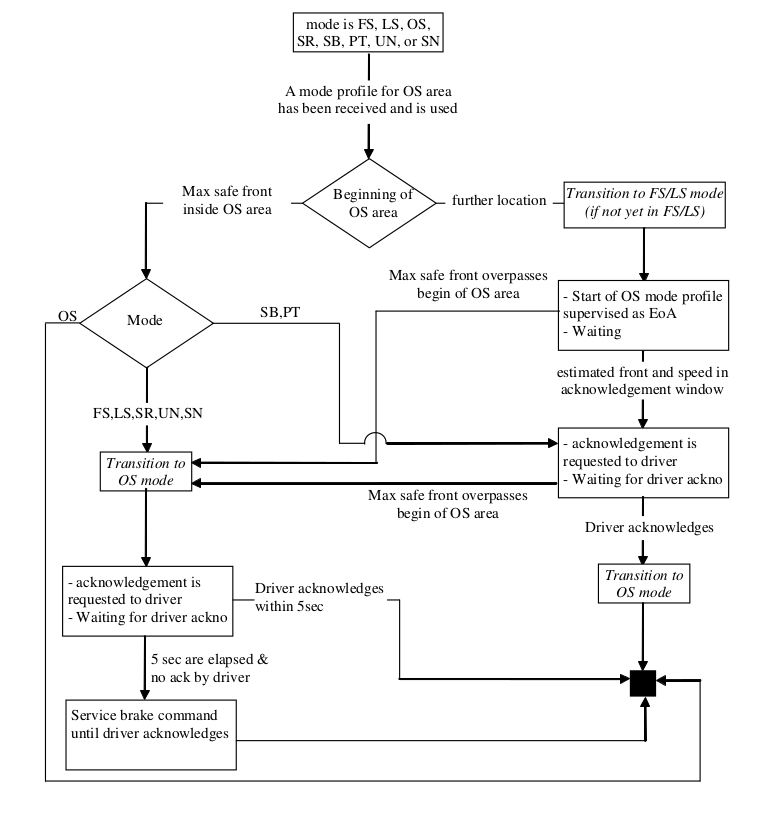
\includegraphics[width=.75\textwidth]{FlowChart}
  \caption{Flowchart for "On-Sight" Procedure~\cite{SRS-026-330}}
  \label{fig:flowchart-OS-mode}
\end{figure}

\subsection{Machine 0 - Basic Flowchart}
\label{sec:machine-0-basic}

The first state machine \bmachine{m0} (see Fig.~\ref{fig:basic-flowchart})
represents an abstract view of the flowchart describing the on-sight procedure
which is shown in §5.9.7 of the SRS~\cite{SRS-026-330} (see
Fig.~\ref{fig:flowchart-OS-mode}).

\begin{figure}[ht]
  \centering
  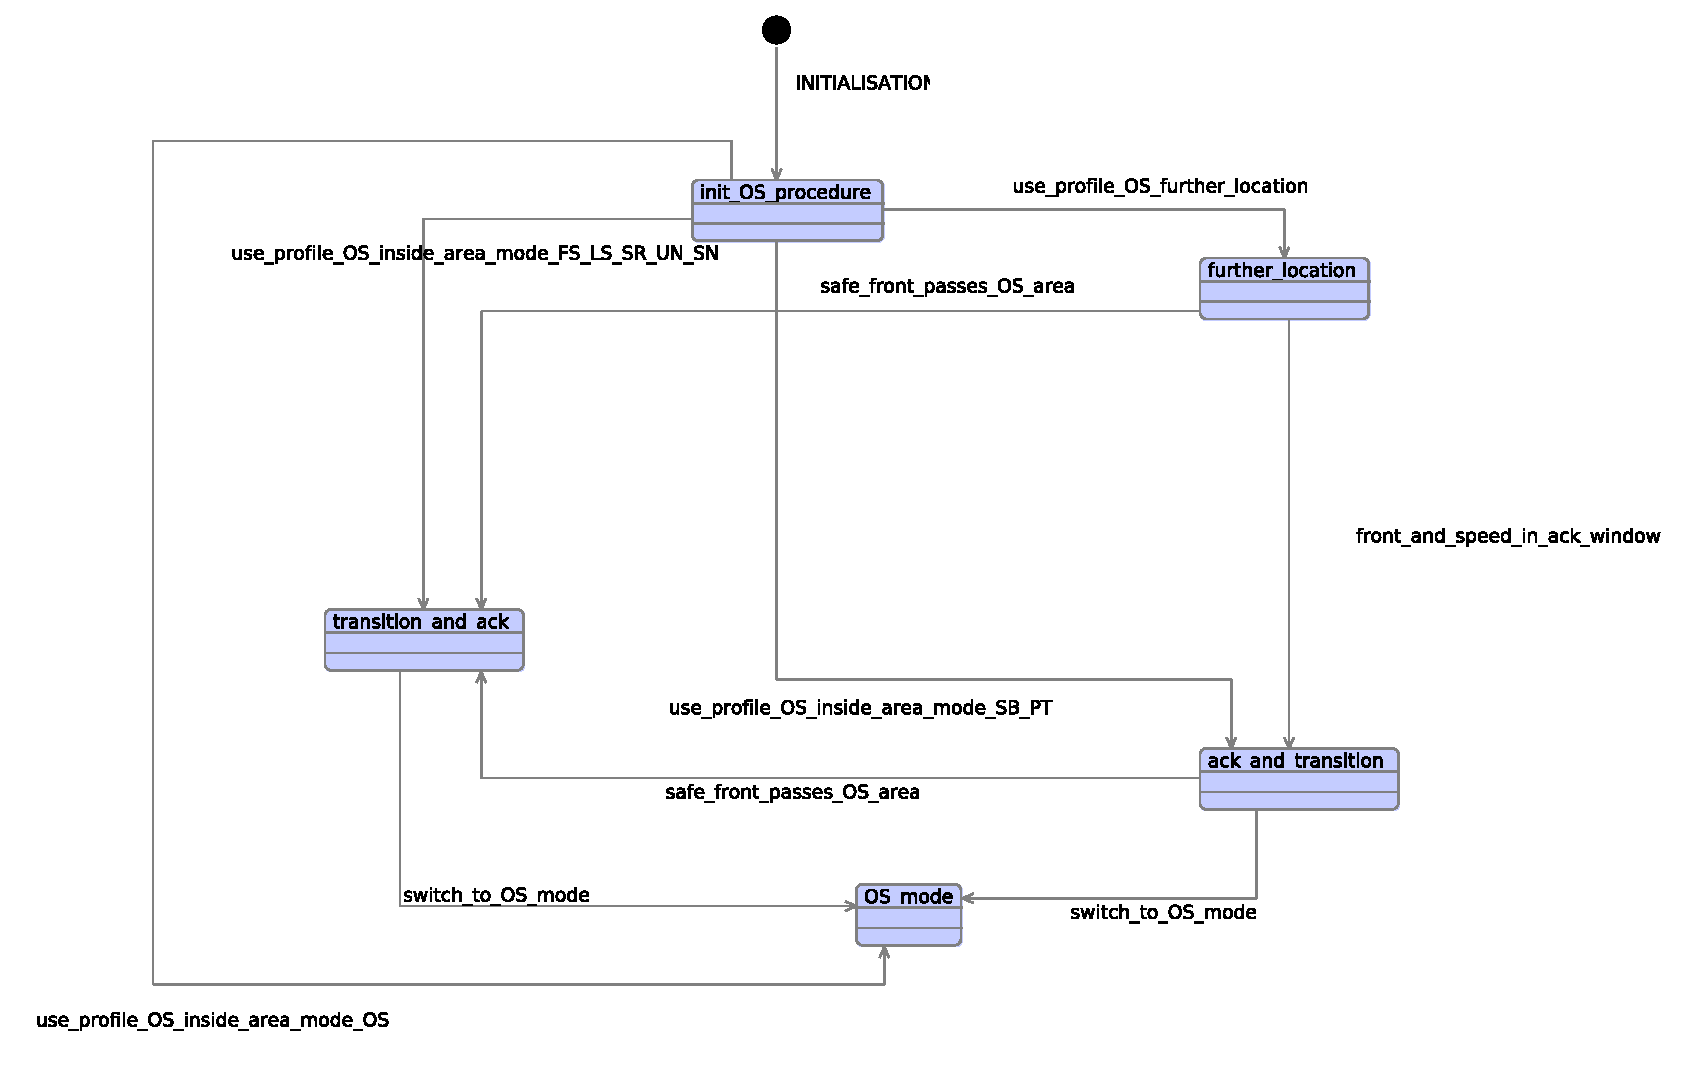
\includegraphics[width=.85\textwidth]{m0_basic_flowchart_on_sight_procedure}
  \caption{Basic Flowchart Representation}
  \label{fig:basic-flowchart}
\end{figure}

The flowchart is translated into a iUML state machine as follows: the initial
state represents the initial situation of the procedure flowchart. The diamonds
of the flowchart represent different cases and are therefore into transitions
with different target states in the state chart. The nodes of the flowchart are
combined for abstraction by combining nodes with multiple incoming flows (or an
initial node) with direct successor nodes.

For example the state \bvar{ack\_and\_transition} can be reached from the
initial state via the event
\bevent{use\_profile\_OS\_inside\_area\_mode\_SB\_PT} and corresponds to the two
lower right nodes of the flowchart. This is justified, as the flow passes two
diamonds in the flowchart, verifying that the i) max safe front of the train is
inside the OS area and ii) the train mode is \bconst{BS} or \bconst{PT}. The
complete model is automatically generated from this state machine. Note
however, that in this abstraction level, there is no concrete notion of train
modes, these appear in the first refinement.


\subsection{Context 0 - Train Modes}
\label{sec:context-0-entities}

The first context \bvar{c0} specifies the possible modes of the train, these are
of type \btype{t\_train\_modes}. There is one Event-B constant for each possible
mode. The constant \bconst{c\_initial\_mode} represents the initial mode of the
train when the procedure on-sight is started. The constant
\bconst{c\_supervision\_mode} is one mode from the supervision modes.

\begin{description}
\SETS
	\begin{description}
		\Item{ t\_train\_modes }
	\end{description}
\CONSTANTS
	\begin{description}
		\ItemY{ c\_FS }{full supervision}
		\ItemY{ c\_LS }{limited supervision}
		\ItemY{ c\_OS }{on sight}
		\ItemY{ c\_SR }{staff responsible}
		\ItemY{ c\_SB }{stand-by}
		\ItemY{ c\_PT }{post-trip}
		\ItemY{ c\_UN }{unfitted}
		\ItemY{ c\_SN }{national system}
		\Item{ c\_initial\_mode }
		\Item{ c\_supervision\_mode }
	\end{description}
\AXIOMS
	\begin{description}
		\nItem{ axm1 }{ partition(t\_train\_modes,\{ c\_FS\} ,\{ c\_LS\} ,\{ c\_OS\} ,\{ c\_SR\} ,		\\\hspace*{6 cm}  \{ c\_SB\} ,\{ c\_PT\} ,\{ c\_UN\} ,\{ c\_SN\} ) }		\nItem{ axm2 }{ c\_initial\_mode \in  \{ c\_FS, c\_OS, c\_PT\}  }		\nItem{ axm3 }{ c\_supervision\_mode \in  \{ c\_LS, c\_FS\}  }	\end{description}
\END
\end{description}




\bibliographystyle{alpha}
\bibliography{openetcs}

\end{document}


%%% Local Variables:
%%% mode: latex
%%% TeX-master: t
%%% End:
